In this chapter I explain my preparatory work, which mainly consists of understanding the problem from the mathematical and research point of view.
First, I explain in detail why measuring robustness of graph metrics is an important and a novel field, describing in detail the work done in ``The Paper'' that this dissertation is based on.
Further I introduce specific definitions of graph metrics and robustness measures that I use in the implementation.


\section{Graphs and metrics}

%The total data (created, captured or replicated) in the world by 2018 was estimated to be 18 zettabytes in 2018 and is expected to reach 175 zettabytes by 2025~\cite{ReinselDigitizationWorldEdge2018}.
Ever-increasing data sources and applications of data science force researchers and data scientists to use tools such as graph theory to model real-world problems.
Graph theory has been used to help solve problems in the field of information technology, engineering, biology, chemistry, social systems, geography, linguistics and many more ~\cite{FouldsGraphTheoryApplications2012}.
Graphs, or networks (nodes and edges), can capture many types of entities and their relations in the real world.
A simple example is a social network in which nodes may represent people and edges represent existence of relationships between pairs of people.

Graph theory proved especially useful when analysing large structures of data that cannot simply be visualised or otherwise analysed by investigating individual entities.
The word \textsl{network} is often used in this context to refer to large instances of graphs stemming from real systems, as opposed to graphs referring more to the mathematical concept itself.
Graph \textsl{statistics} (e.g. size, average degree, diameter, radius) have been invented to help mathematically describe properties of arbitrarily large graphs, such as betweenness centrality.
Further, graph \textsl{metrics} (such as betweenness centrality, closeness centrality, eccentricity) quantify properties of individual nodes.
For example a person represented by a node with high closeness centrality score is considered to be \textsl{closer} to others in terms of number of hops needed, in other words can spread information in the network faster.


\section{Introduction to confidence}

Statistical significance, confidence scores, confidence intervals, error ranges, all signal or approximate the extent to which the observed result is reliable.
Some confidence values are a direct probability that an error is present, given the available evidence (such as a statistical significance when rejecting a null hypothesis).
Other measures such as error ranges or standard deviations estimate how much off a numerical value may be.

Networks obtained from the real-world by experiments, observations, or deductions,may contain errors too, such as missing nodes or edges, false positives, uncertain nodes or edges, falsely aggregated nodes.
Network errors may stem from measurement errors, approximations, lack of knowledge, lack of experimental evidence or thresholding of scored networks~\cite{Wang2012,MarsdenNetworkDataMeasurement1990,JonesChallengesLimitationsQuantifying2010}.
These errors may then propagate and cause errors in graph metrics.

Error measures are important to assess how precise or confident an experiment or an observation is.
A research result without examining its precision or confidence can be considered incomplete.\citeneeded{}

\parskip

However, can we measure precision or confidence of graph metrics?
If an outcome is based on evaluating metrics on graphs which are themselves imprecise or possibly have errors in the structure, how can we assess the confidence or precision of such result?
\unimportant{Helping to answer these questions is the motivation behing building \graffs.}

A number of attempts already tried to assess robustness or stability properties of graph metrics.
Examples are analysing impact of errors on centrality measures in random networks~\cite{BorgattiRobustnessCentralityMeasures2006} or, more specifically, evaluating reproducibility of metrics on multi-temporal scans of human brain using coefficient of variation (CV), the repeatability coefficient (RC) and the intra class correlation (ICC)~\cite{VaessenEffectReproducibilityDifferent2010,DennisTestRetestReliabilityGraph2012}.
A significant amount of research analysing reproducibility of metrics in uncertain brain networks appeared around 2011, summarised in~\cite{TelesfordExplorationGraphMetric2013}.
\unimportant{The latest research led to development of methods for analysis of such uncertain data, estimating a ground-truth network structure from imperfect data~\cite{Martin2016,Newman2018}, and even a method to mitigate sensitivity of metrics on the selection of a threshold in scored networks~\cite{Drakesmith2015}.}


\section{The Paper}

This dissertation project is based on, and extending the ideas from the paper by Bozhilova et al.: \textsl{Measuring rank robustness in scored protein interaction networks}~\cite{Bozhilova2019}.
In my work I refer to~\cite{Bozhilova2019} as \textsl{The Paper}.

The Paper is one of the most recent researches on metric robustness.
The study demonstrates instability of some graph metrics on thresholded protein networks and proposes ways to quantify robustness of graph metrics in such networks.

\subsection{Protein networks}

Protein interaction networks (PINs), also called protein-protein interaction (PPI) networks, are an example of a prominent research field relying on graph theory.
Nodes in protein networks represent proteins present in cells of organisms and edges represent interactions between them, often labelled to convey additional information.

Studying them helps in understanding physiology of biological cells and developing drugs as they generally affect protein interactions.
For example, highly connected proteins and hubs of proteins in a cell are shown to be most essential for its survival~\cite{JeongLethalityCentralityProtein2001,HeWhyHubsTend2006}.

Protein networks have a specific structure: nodes represent proteins and weighted (or scored) edges represent the presence of interactions between proteins.
It is assumed that such interactions are mutual, therefore the formed graph is undirected.

\begin{figure}[ht]
    \vspace*{-3mm}
    \tikzset{every picture/.style={line width=0.75pt}} %set default line width to 0.75pt
    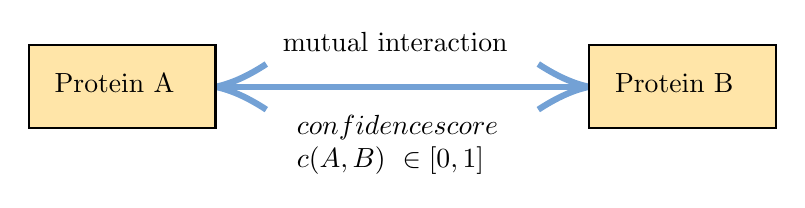
\begin{tikzpicture}[x=0.75pt,y=0.75pt,yscale=-1,xscale=1]
        %uncomment if require: \path (0,136); %set diagram left start at 0, and has height of 136

        %Straight Lines [id:da5202946805882411]
        \draw [color={rgb, 255:red, 115; green, 161; blue, 213 }  ,draw opacity=1 ][fill={rgb, 255:red, 0; green, 0; blue, 0 }  ,fill opacity=1 ][line width=2.25]    (114,40) -- (286,40) ;
        \draw [shift={(290,40)}, rotate = 180] [color={rgb, 255:red, 115; green, 161; blue, 213 }  ,draw opacity=1 ][line width=2.25]    (24.48,-10.98) .. controls (15.57,-5.15) and (7.41,-1.49) .. (0,0) .. controls (7.41,1.49) and (15.57,5.15) .. (24.48,10.98)   ;
        \draw [shift={(110,40)}, rotate = 0] [color={rgb, 255:red, 115; green, 161; blue, 213 }  ,draw opacity=1 ][line width=2.25]    (24.48,-10.98) .. controls (15.57,-5.15) and (7.41,-1.49) .. (0,0) .. controls (7.41,1.49) and (15.57,5.15) .. (24.48,10.98)   ;
        %Shape: Rectangle [id:dp8315683426496481]
        \draw  [fill={rgb, 255:red, 255; green, 229; blue, 168 }  ,fill opacity=1 ] (20,20) -- (110,20) -- (110,60) -- (20,60) -- cycle ;
        %Shape: Rectangle [id:dp6227729030936355]
        \draw  [fill={rgb, 255:red, 255; green, 229; blue, 168 }  ,fill opacity=1 ] (290,20) -- (380,20) -- (380,60) -- (290,60) -- cycle ;

        % Text Node
        \draw (31,32) node [anchor=north west][inner sep=0.75pt]   [align=left] {Protein A};
        % Text Node
        \draw (301,32) node [anchor=north west][inner sep=0.75pt]   [align=left] {Protein B};
        % Text Node
        \draw (141,12) node [anchor=north west][inner sep=0.75pt]   [align=left] {mutual interaction};
        % Text Node
        \draw (141,50.4) node [anchor=north west][inner sep=0.75pt]    {$ \begin{array}{l}
                                                                              \text{confidence score}\\
                                                                              c( A,B) \ \in [ 0,1]
        \end{array}$};
    \end{tikzpicture}
    \caption{Schematic of an interaction between two proteins}
    \vspace*{-2mm}
\end{figure}


\subsection{Confidence scores}

The weight of each edge in protein networks represents a confidence score which may be a value, or a set of values, describing some sort of \textsl{likelihood} that the given interaction is true, given the available evidence.
They do \textsl{not} indicate the strength or intensity of the interaction (which would be a different property).

As an example, the STRING database~\cite{Szklarczyk2019} used in The Paper is an open collection that contains known and predicted protein-protein interactions.
It provides confidence scores for edges, indicating how likely the dataset authors consider an interaction to be true, given the available evidence.
Databases HitPredict~\cite{LopezHitPredictVersionComprehensive2015} and IntAct~\cite{OrchardMIntActProjectIntAct2014} and others use a similar approach.

Edges in the STRING database have confidence scores for various types of evidence, such as scientific experiments, genetic observations (gene fusions, gene co-occurrence), statistical predictions, text mining of scientific articles, or existing knowledge (other available protein interaction databases).
An approximation of an overall confidence score is calculated for each edge (illustrated in \autoref{fig:string_network_image}).
The Paper, as well as my dissertation, use only the overall confidence score and do not focus on the biological details of each evidence type.

\afterpage{
    \begin{figure}
        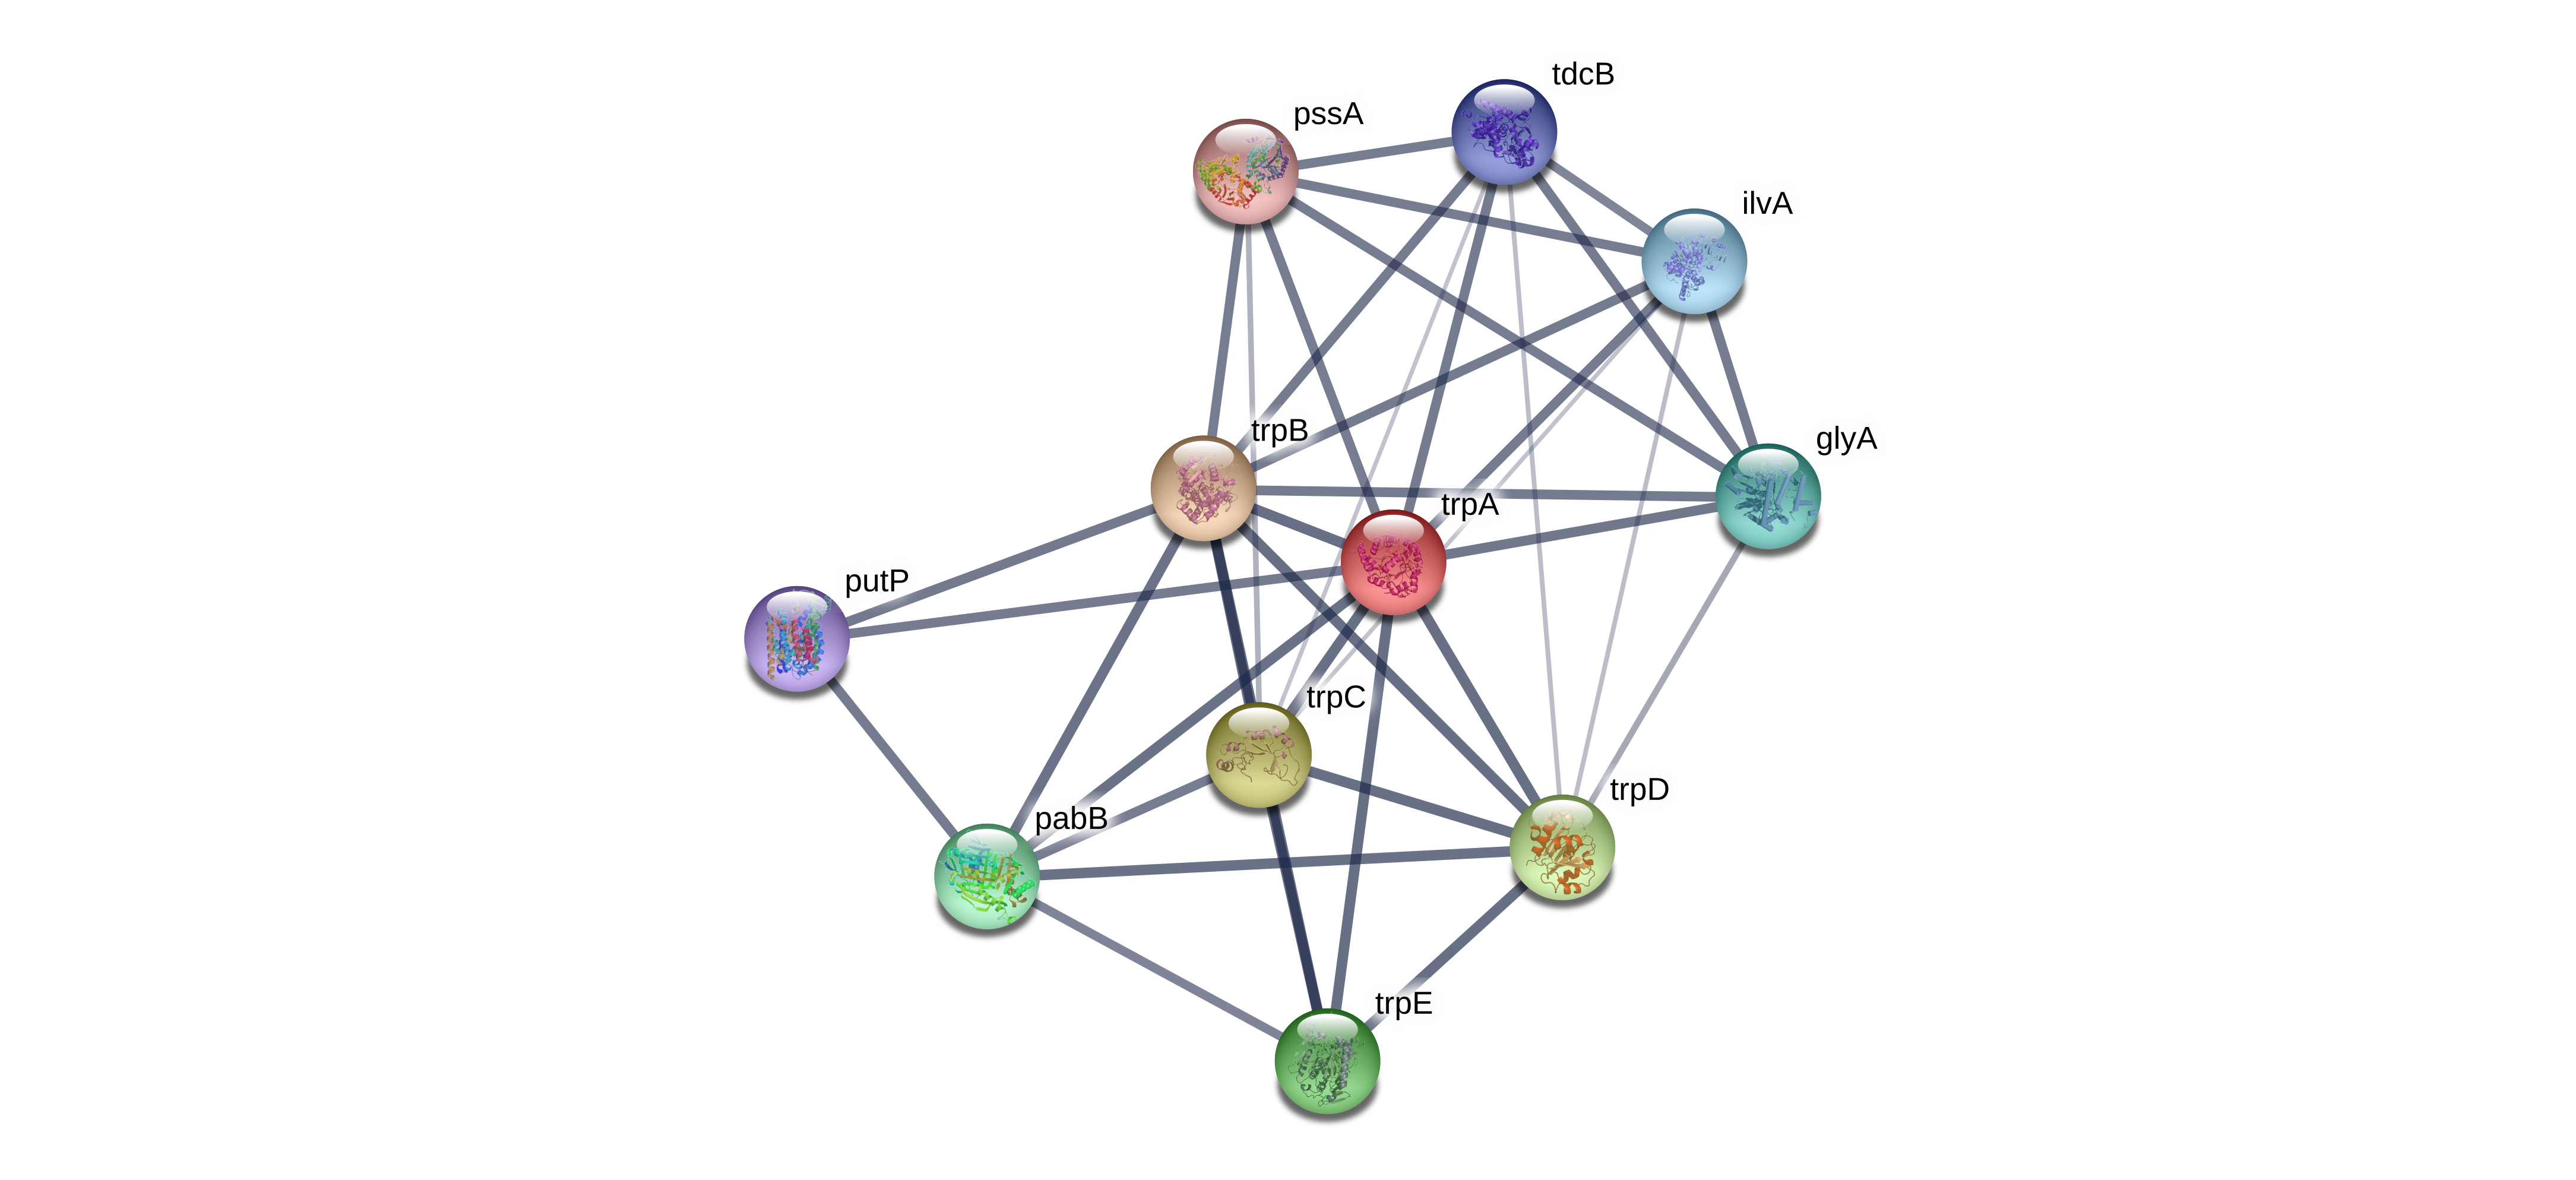
\includegraphics[height=7cm]{string_network_image.png}
        \caption[Protein-protein interaction network visualised by the STRING database~\cite{Szklarczyk2019}.
        Edge thickness indicates the overall confidence score, i.e. the strength of data support.]%
        {Protein-protein interaction network visualised\protect\footnotemark{} by the STRING database~\cite{Szklarczyk2019}.
        Edge thickness indicates the overall confidence score, i.e. the strength of data support.}
        \label{fig:string_network_image}
    \end{figure}
    \footnotetext{Available at \url{https://version-11-0.string-db.org/cgi/network.pl?networkId=8lbbIYSrLfZG}}
}


\subsection{Network thresholding}

\begin{figure}
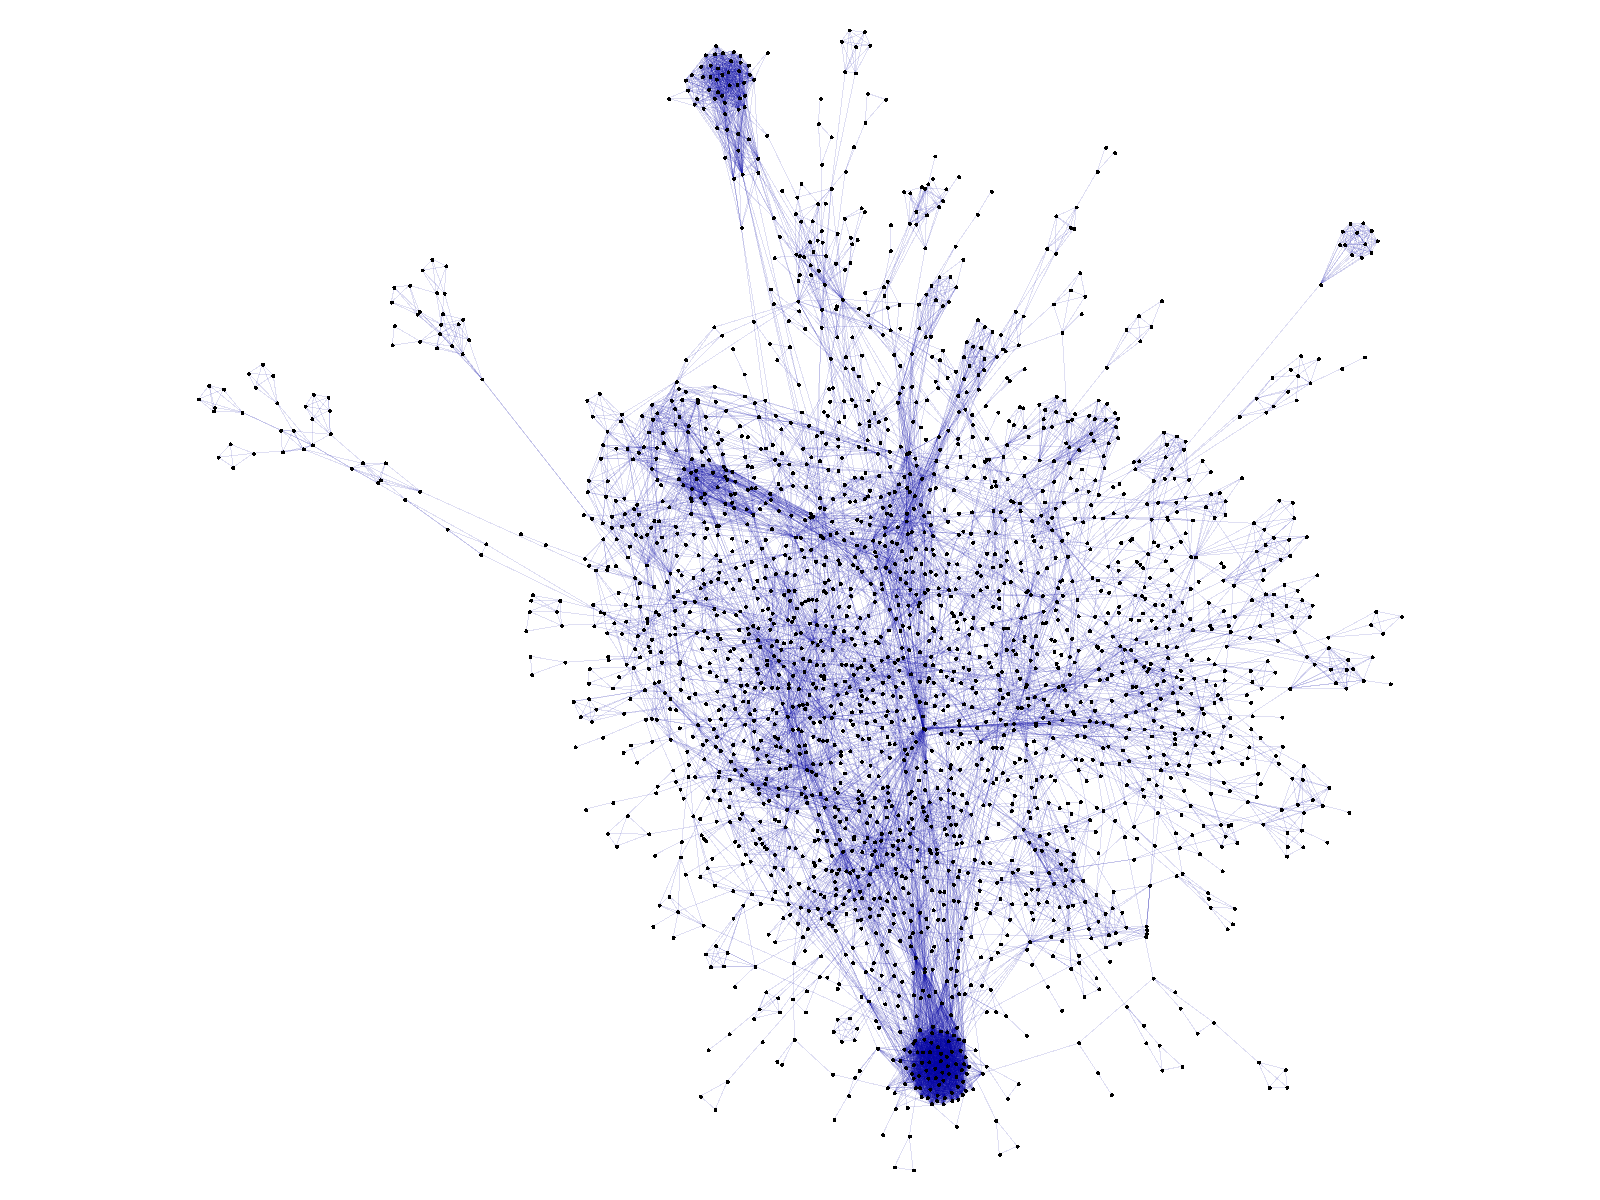
\includegraphics[height=8cm]{ecoli_giant_at_900.png}
\caption{An interaction network of proteins from the \textit{Escherichia coli} organism from the STRING database, thresholded at the $0.9$ score (high confidence). Only nodes of the giant component are shown.}
\label{fig:ecoli_giant_at_900}
\end{figure}


When researching protein interactions, in practice, researchers choose a \textbf{threshold} and then form a protein interaction network from the database considering only interactions (edges) whose confidence score is greater than the selected threshold, to only take into account interactions of sufficiently high quality.
Thresholding edges of sufficient confidence is a common step before further graph analysis.

\autoref{fig:ecoli_giant_at_900} shows an example of a protein network taken from the STRING database, containing proteins of the \textit{Escherichia coli} organism.
Only edges with score of $0.9$ corresponding to the ``highest confidence'' level (on the scale from $0$ to $1$) were retained, and only the giant connected component of it is shown.
That yields a graph with 2382 nodes and 12071 edges.

\todo{Histogram of edge confidence of a graph such as \textsl{ecoli}}

\subsection{Metric robustness}

However, as The Paper remarks, the analysis based on metric evaluation can be sensitive to the choice of the threshold.
If a node metric is to be useful for extracting biological signal, it should lead to similar results across networks obtained at different reasonable confidence score thresholds.
Hence, the point of studying metric robustness or \textsl{stability} is a way to assess how reliable the results are on a graph derived from a given threshold.

When measuring robustness of node metrics, numerical values of metrics will undoubtedly depend on the chosen threshold, for example the degree and the clustering coefficient of each node will indeed monotonically decline with declining density of the network, which monotonically declines as we increase the confidence threshold.
For this reason, the point of The Paper is to assess a robustness of graph metrics based on the \textbf{rankings} of nodes induced by each metric (where ranking is just a total preorder of the nodes based on the metric values).

\subsubsection*{Rank robustness}

The Paper introduces three different measures assessing robustness of node metrics (all are further explained later):
\begin{itemize}
    \item rank continuity (comparing highly ranked nodes at similar thresholds),
    \item rank identifiability (comparing ranks at various thresholds and the overall ranking),
    \item rank instability (quantifying variation of ranks of top 1\% of nodes).
\end{itemize}
All three measures are based on rankings of nodes induced by node metrics, and not on the exact values, to mitigate the density bias described above.

The Paper studies robustness of 25 different \textsl{node} metrics only, i.e. graph metrics which return one numerical value per node.


\section{Mathematical background}\label{sec:math_background}

In this section I review background material on graph theory and examining graph metric robustness, and fix terms I will use later to avoid ambiguity in further chapters.

In particular, this section will focus introducing high-level concepts of:
\begin{itemize}
    \item relevant bits of graph theory
    \item graph metrics
    \item ranking
    \item metric robustness
\end{itemize}

\subsection{Graphs}

Graphs (or networks) from graph theory usually consist of \textit{components} (or nodes, vertices) and \textit{links} between them (edges).
Some definitions in this subsection are based on the book \textsl{A first course in network theory}\cite{Estrada2017}.

\begin{definition}[Graph]
    Let $V$ be a finite set of $n$ nodes (or vertices), and let $E \subseteq V \times V$ be a set of edges.\\
    A \textbf{graph} $G$ is a pair $(V, E)$.\\
    $V$ is the \textbf{node set} of $G$, and $E$ is the \textbf{edge set} of $G$.
\end{definition}

Real-world data (or datasets) in the form of graphs are also called \textbf{networks}.
Still, I may interchange the words \textsl{graph}, \textsl{network} and \textsl{dataset}, but generally:
\begin{itemize}
    \item \textsl{dataset} is data stored in its raw form, such as a file downloaded from the Internet
    \item \textsl{network} is the real-world graph-like data conveyed by a dataset
    \item \textsl{graph} is a hypothetical structure, also a mathematical interface or representation that algorithms work with
\end{itemize}

\begin{definition}[Graph properties]
    \begin{itemize}[leftmargin=*]
        \item $G$ is \textbf{reflexive} iff $\forall v \in V.\ (v, v) \in E$
        \item $G$ is \textbf{anti-reflexive} iff $\forall v \in V.\ (v, v) \notin E$
        \item $G$ is \textbf{undirected} (or equally \textbf{symmetric}) iff $\forall v_1, v_2 \in V.\ (v_1, v_2) \in E \Rightarrow (v_2, v_1) \in E$
        \item $G$ is \textbf{directed} iff it is not undirected
        \item $G$ is a \textbf{simple graph} iff it is undirected and anti-reflexive
    \end{itemize}
\end{definition}

Graphs I use in this project are all \textsl{simple graphs} (unless stated otherwise), i.e. edges are undirected (or bi-directional), and always span two different nodes.

\begin{wrapfigure}[11]{R}{0.31\textwidth}
\vspace*{-10mm}
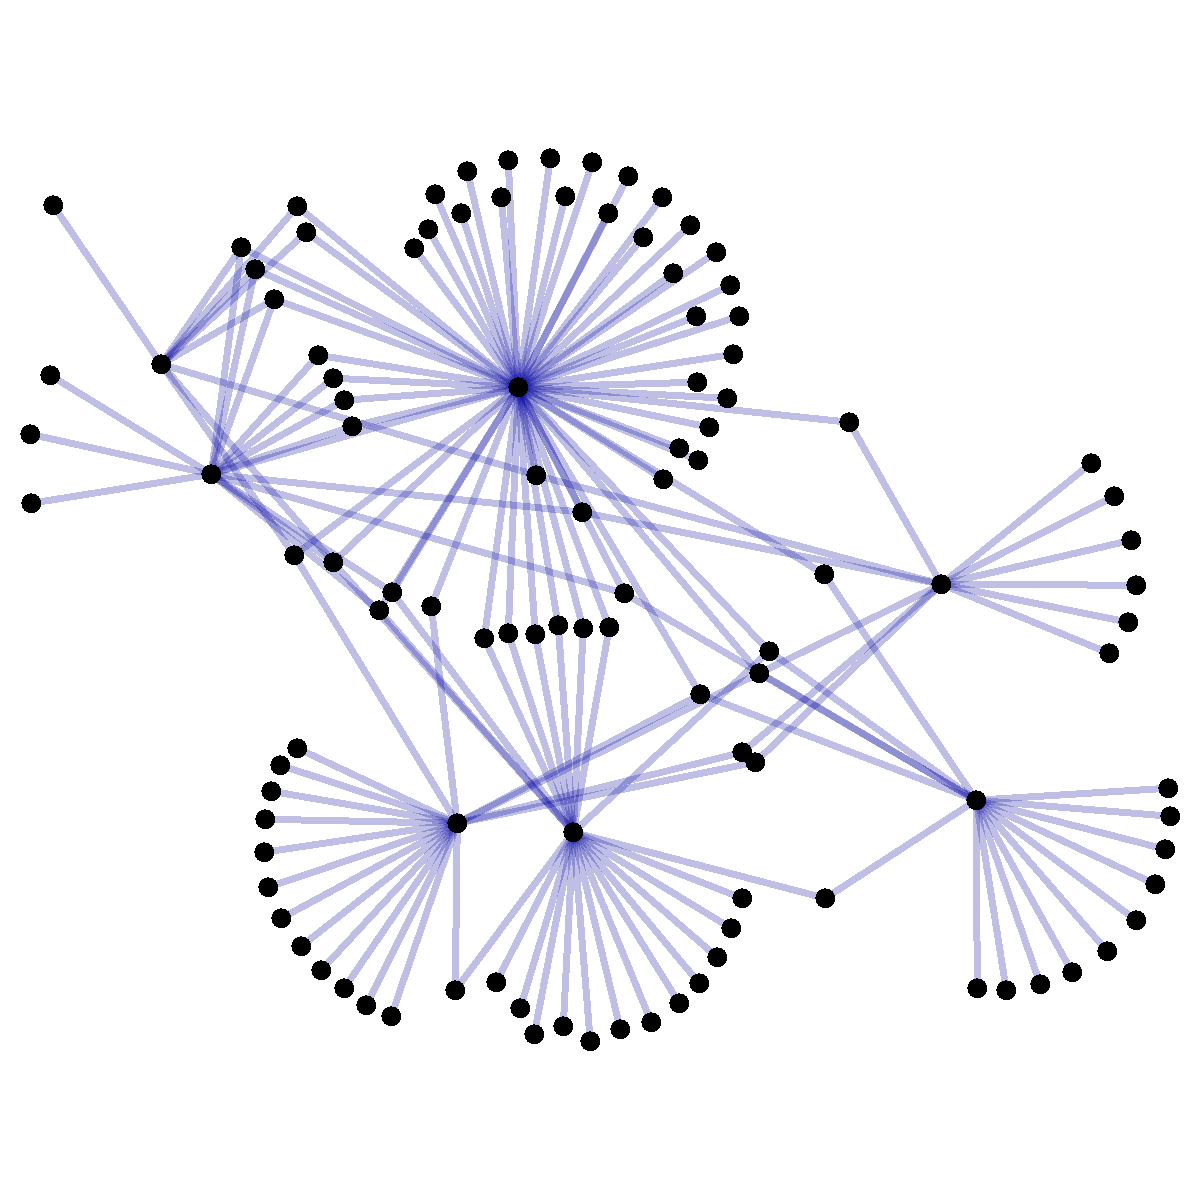
\includegraphics[width=\linewidth]{simple_graph.png}
\vspace*{-10mm}
\caption{A small example of a \textsl{connected} \textsl{simple} graph (\textsl{undirected} and \textsl{anti-reflexive}).}
\label{fig:simple_graph}
\end{wrapfigure}


\autoref{fig:simple_graph} is an illustration of a connected simple graph with 110 nodes and 151 edges.
I used graphs like this for testing purposes when developing \graffs.

\begin{definition}[Relations on graphs]
    \begin{itemize}[leftmargin=*]
        \item $G' = (V', E')$ is a \textbf{subgraph} of $G = (V, E)$ iff $V' \subseteq V$ and $E' \subseteq E$
        \item Let $G_1 = (V_1, E_1)$ and $G_2 = (v_2, E_2)$, then $G_1 \cup G_2 = (V_1 \cup V_2, E_1 \cup E_2)$ is the \textbf{union} of the two graphs, and $G_1 \cap G_2 = (V_1 {\cap} V_2, E_1 {\cap} E_2)$ is the \textbf{intersection} of the two graphs.
    \end{itemize}
\end{definition}

\begin{definition}[Node adjacency]
    \begin{itemize}[leftmargin=*]
        \item In an undirected graph, $v_1$ is \textbf{adjacent} to $v_2$ iff $(v_1, v_2) \in E$
        \item A \textbf{loop} is an edge of the form $(v, v)$.
        Note that simple graphs have no loops.
        \item Define $\deg^-(v) = \left\lvert \Set{v' \in V}{(v', v) \in E} \right\rvert$ to be the \textbf{indegree} of $v$, and $\deg^+(v) = \left\lvert \Set{v' \in V}{(v, v') \in E} \right\rvert$ to be the \textbf{outdegree} of $v$, in other words, the number of incoming and outcoming edges, respectively.
        If the graph is undirected, then $\deg^-(v) = \deg^+(v) = \deg(v)$ is called \textbf{degree}.
        \item For $G = (V, E)$ with $V = \integersto{n}$, define $A = (a_{ij})$ to be the \textbf{adjacency matrix} of $G$ where
        \[ a_{ij} = \begin{cases}
                        1, & \textnormal{if}\ (i, j) \in E \\
                        0, & \textnormal{if}\ (i, j) \notin E
        \end{cases} \]
        for $1 \leq i, j \leq n$.

        Note that adjacency matrix of undirected graph is symmetric.
    \end{itemize}
\end{definition}

\begin{definition}[Connectedness]
    \begin{itemize}[leftmargin=*]
        \item $u, v$ are \textbf{connected nodes} is there exists a path between $u, v$ in $G$, i.e. if $(A^k)_{uv} = 1$ for some $k\in \mathbb{N}$.
        \item $G = (V, E)$ is \textbf{connected graph} if $\forall v_1, v_2 \in V. v_1, v_2$ are connected nodes.
        \item A subgraph $G' \subseteq G$ is a \textbf{(connected) component} iff $G'$ is a maximal connected subgraph of $G$.

        Note that all components of a graph are disjoint, therefore each node belongs to exactly one component.
    \end{itemize}

    \item A \textbf{giant component} of a graph is a single component that has more nodes than any other component of the graph.

    Note that a giant component may not exist, if more components have maximum number of nodes.
\end{definition}

\begin{figure}
\vspace*{-4mm}
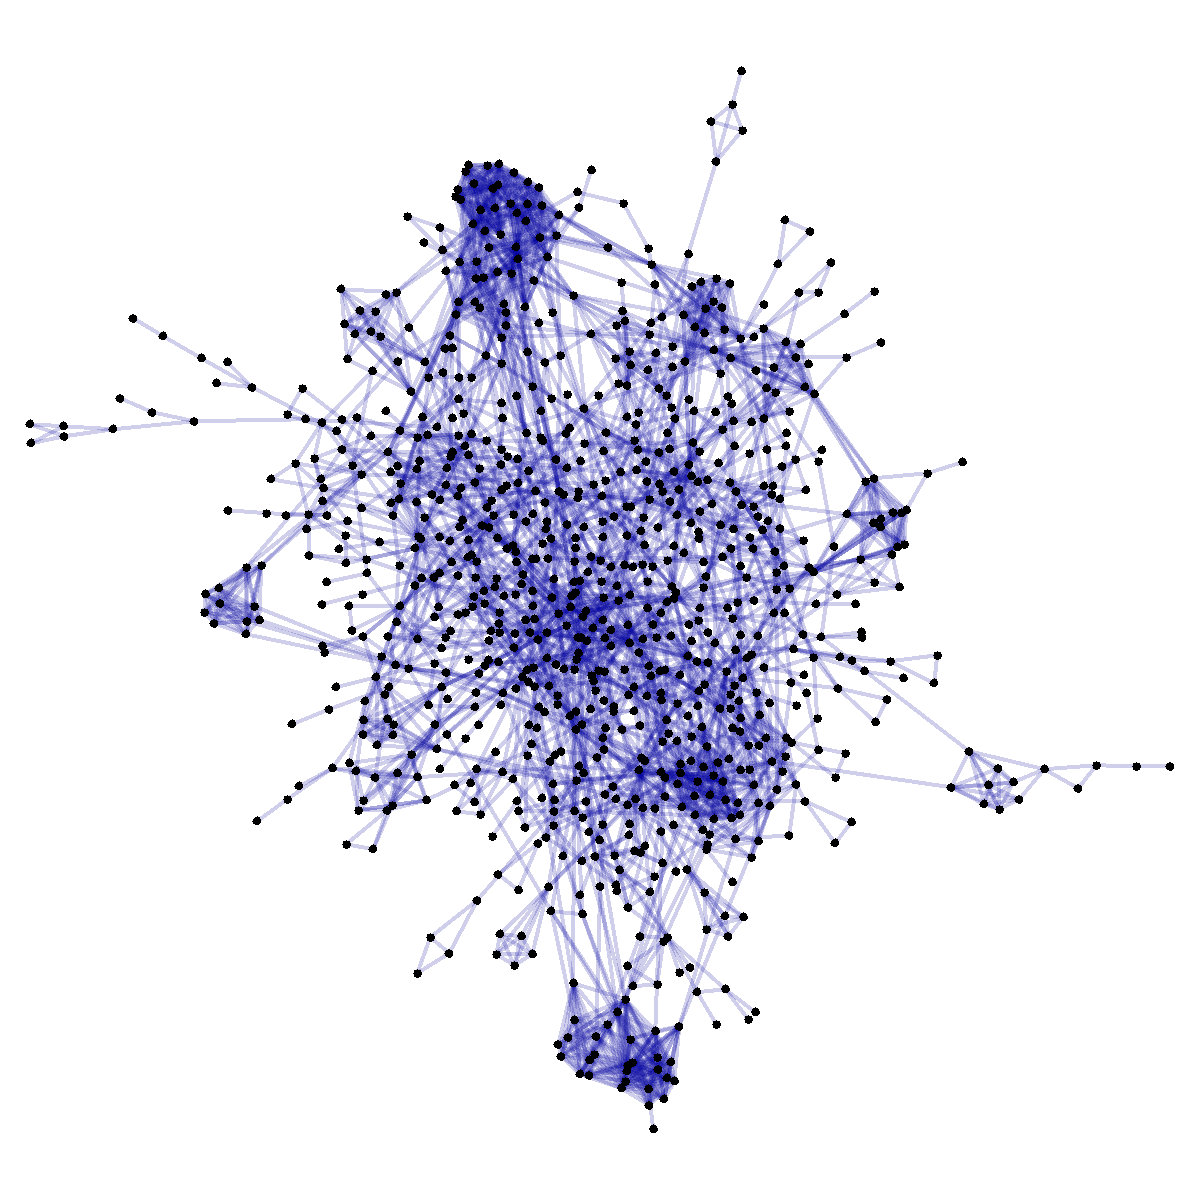
\includegraphics[height=6cm]{disconnecting_graph.png}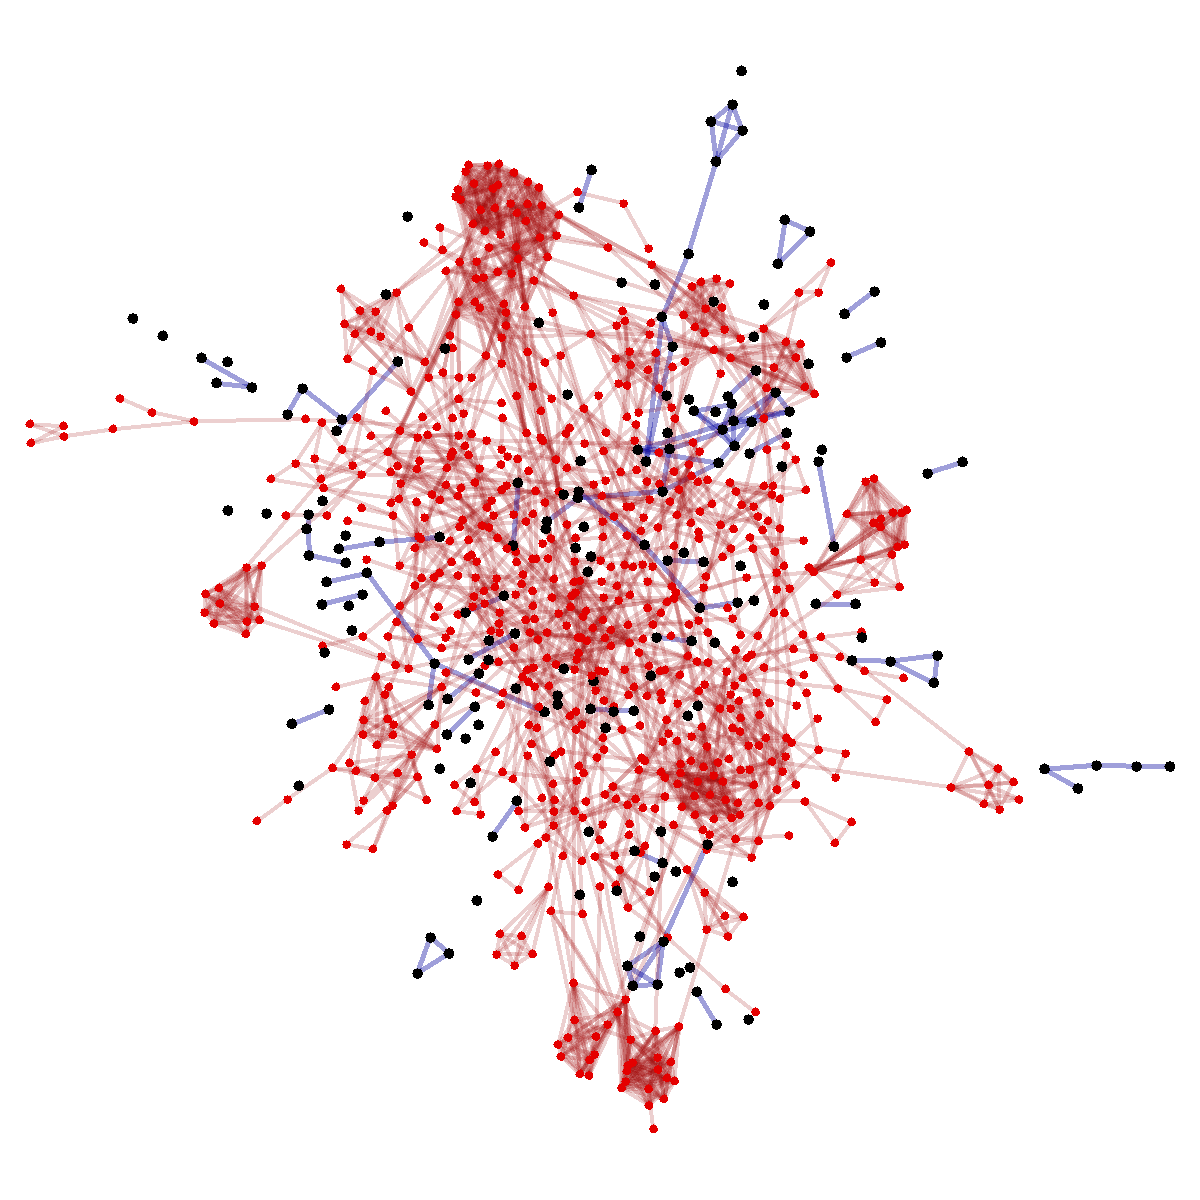
\includegraphics[height=6cm]{disconnecting_graph2.png}
\vspace*{-4mm}
\caption{Illustrated is how thresholding (a subgraph of) a protein network (left) results in one giant component (red) and multiple small disconnected components.
The left is a certain subgraph of the \textit{ecoli} dataset (all edges with confidence $>0.4$), the right graph has only edges with confidence $>0.5$.}
\label{fig:disconnecting_graph}
\end{figure}


Most of real-world networks (such as social networks, citation networks and even protein interaction networks) contain a single giant component, and some small isolated components.
For example, in \autoref{fig:disconnecting_graph}, the red nodes form a giant component of the graph.


%\subsubsection{Networks}
%
%Moving towards real-world data, graphs often emerge from a certain source in the world.
%Just a few examples of the data possibly represented by graphs include social networks, road networks, computer networks, protein interaction networks, citation networks, web networks and so on.
%In this work I distinguish graphs and networks, although I may sometimes interchange these two.
%
%\begin{definition}[Network]
%    A \textbf{network} is a graph whose nodes or edges can have attributes $\textnormal{attr}_v, \textnormal{attr}_e : \Sigma^* \rightarrow \mathbb{U}$ for some set of possible identifiers $\Sigma^*$ (such as a language over an alphabet $\Sigma$) and a value domain $\mathbb{U}$ (such as $\mathbb{R}$ or $\mathbb{R}^2$)
%\end{definition}
%
%Graphs and networks allow capturing the same structure, however, the main difference is that nodes of a network are \textit{identifiable}, while we rarely consider \textit{identity} of graph nodes.
%%This is because nodes and edges of graphs coming from real-world are often (nearly) isomorphic to real-world objects and relations between them.
%There may be either an exact or inexact matching between nodes/edges in the graph and objects/relations in the real world where the data came from (depending on whether the dataset is an approximation of the world).
%I will often use networks when describing knowledge of the world.
%

\subsection{Graph metrics}

Metrics are essentially functions of graphs that assign a value to each node.
Metrics are used to quantify various properties of graphs, identifying important nodes in different contexts, describing graph structures, comparing different graphs and more.
Metrics are crucial in analysing graphs of ever-growing real-world data.

Mathematically speaking, if $\mathbb{G}$ is the set of all graphs $G = (V, E)$ with $V \subset \mathbb{V}$, then we can define the domain of metrics to be generally functions of graphs:
\begin{equation}
    \label{eq:metric_type_def}
    \mathbb{M} \eqdef \mathbb{G} \Rightarrow (\mathbb{V} \Rightarrow \mathbb{R})
\end{equation}

Evaluation of a metric on a graph then results in a \textsl{mapping} of nodes to real numbers.
Therefore, for some metric $M \in \mathbb{M}$, some graph $G = (V, E)$, and a node $v \in V$:
\begin{align}
    &M(G) : \mathbb{V} \rightarrow \mathbb{R}\\
    &M(G)(v) \in \mathbb{R}
\end{align}

However, for convenience, in the notation the graph argument is often left out when it is understood which graph the metric is applied to, resulting in $M(v) \in \mathbb{R}$.

\parspace

In this section I describe some of the metrics that are most significant for analysing protein interaction networks, and other graphs used in this project.
The set of these metrics and their specific definition is based on The Paper\cite{Bozhilova2019}, and on~\cite{MartinHernandez2011}.

All metrics below are defined for \textsl{undirected} graphs.

\subsubsection{Centralities}

One of the simplest metrics calculates the \textsl{degree} of each node, which is often considered a centrality measure (indicating that nodes with higher degree are more important in the network).

\begin{definition}[Degree (centrality)]
    For a graph $G = (V, E)$, define degree centrality $DC : V \rightarrow \mathbb{N}$:
    \begin{equation*}
        DC(v) \eqdef \deg(v) = \left\lvert \Set{v' \in V}{(v', v) \in E} \right\rvert
    \end{equation*}
\end{definition}

Another one of the most common centrality measures, \textsl{betweenness centrality}, is calculated for each node $v$ as the number of all shortest paths passing through that node, for all pairs of nodes.
If there are multiple shortest paths between a pair of nodes, the fraction of those passing through $v$ are considered.

\begin{definition}[Betweenness centrality]
    For a graph $G = (V, E)$, define betweenness centrality $B : V \rightarrow \mathbb{R}$:
    \begin{equation*}
        B(v) \eqdef \sum_{\substack{s,t \in V \\ s \ne v \ne t}} \frac{ \sigma_{st}(v) }{ \sigma_{st} }
    \end{equation*}
    where $\sigma_{st}$ is the number of shortest paths between $s$ and $t$, and $\sigma_{st}(v)$ is the number of those that pass through $v$.
\end{definition}

\textsl{Closeness centrality} of a node $v$ is the reciprocal value of the sum of $d(v, i)$, the distances from that node to all other nodes $i$ in the graph.
It measures the reciprocal of the \textsl{farness} of each node to other nodes.
Nodes with higher closeness centrality are \textsl{closer} to all other nodes.

\begin{definition}[Closeness centrality]\label{def:closeness_centrality}
    \[CC(v) \eqdef \frac{1}{\sum_{i \neq v} d(v, i)}\]
\end{definition}

This is well-defined for connected graphs, however, $d(v, i)$ is undefined if $v, i$ belong to two different components of the graph.
For disconnected graphs, I set $d(v, i) = \left\lvert V \right\rvert$ to follow the approach in The Paper.

\begin{figure}
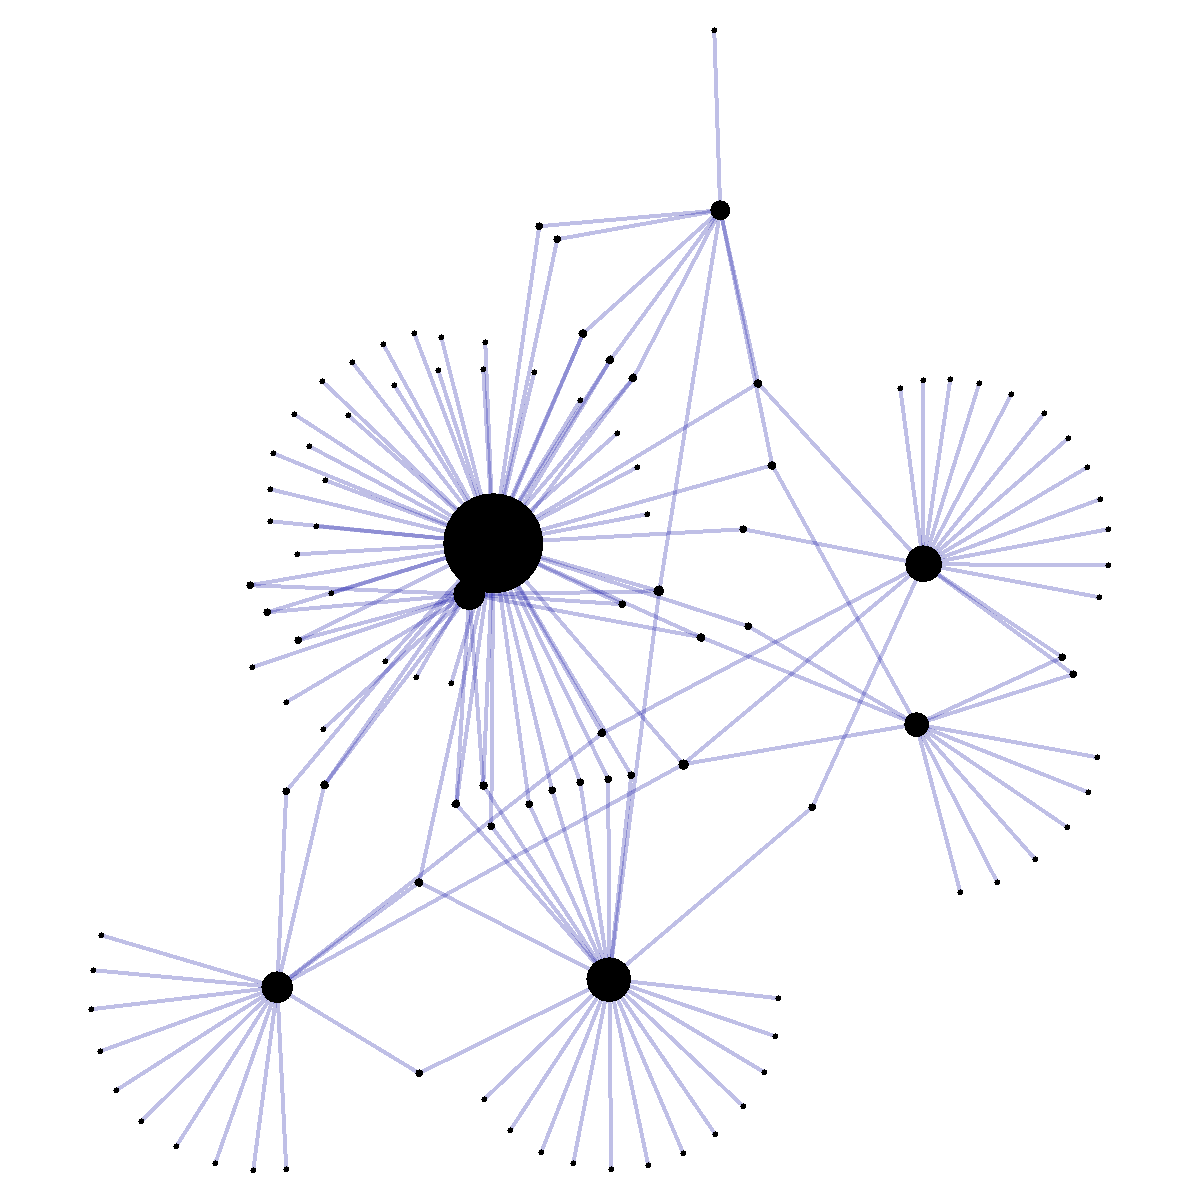
\includegraphics[height=5cm]{simplegraph_by_some_metrics.png}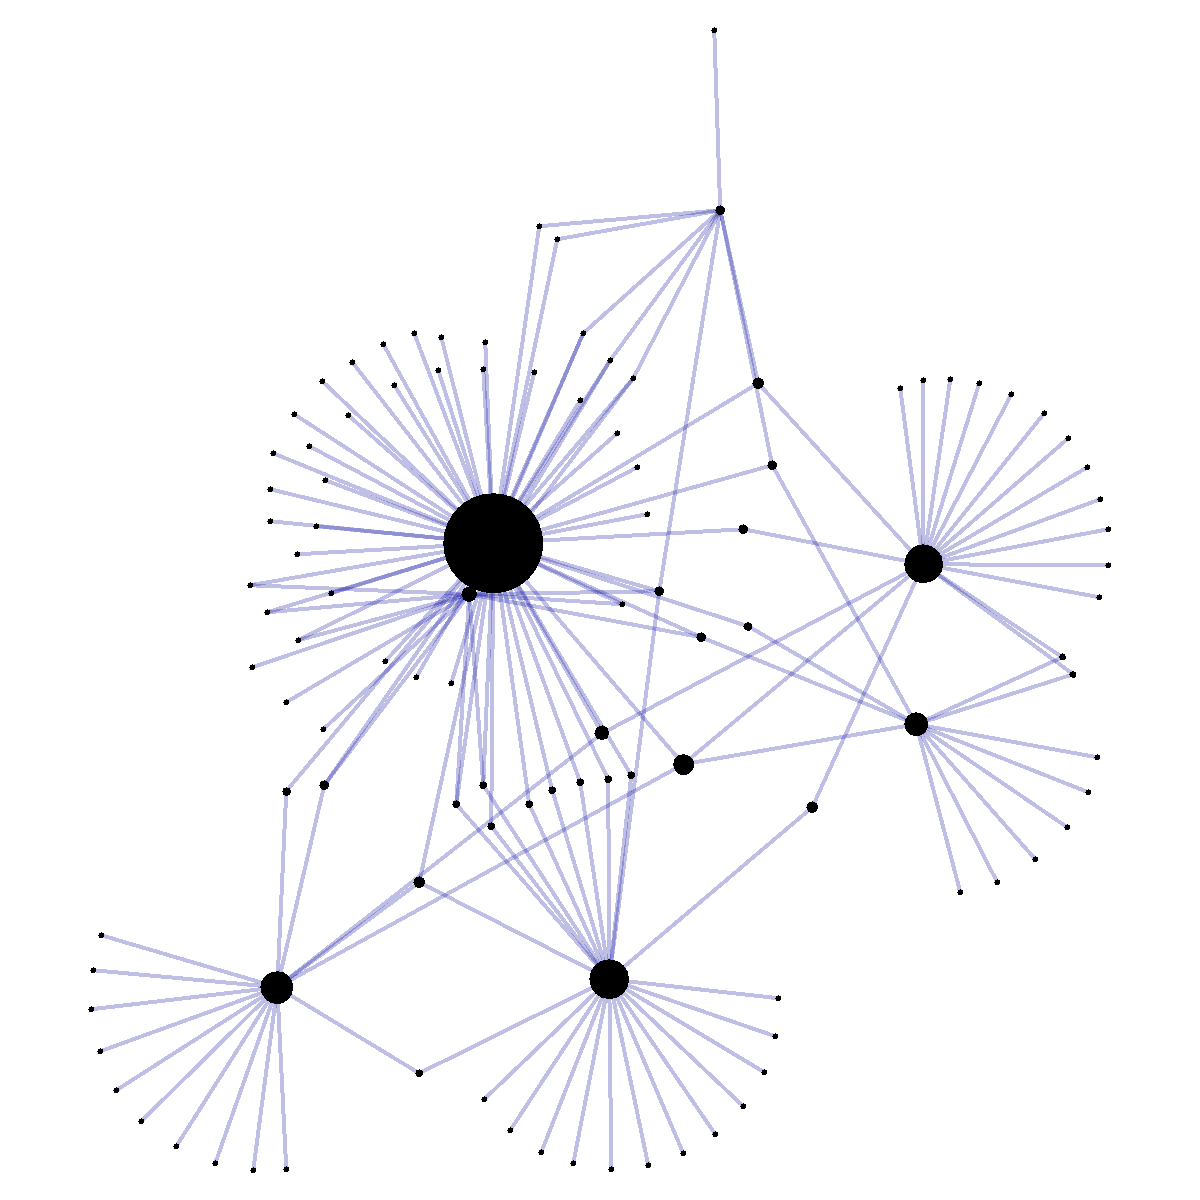
\includegraphics[height=5cm]{simplegraph_by_some_metrics2.png}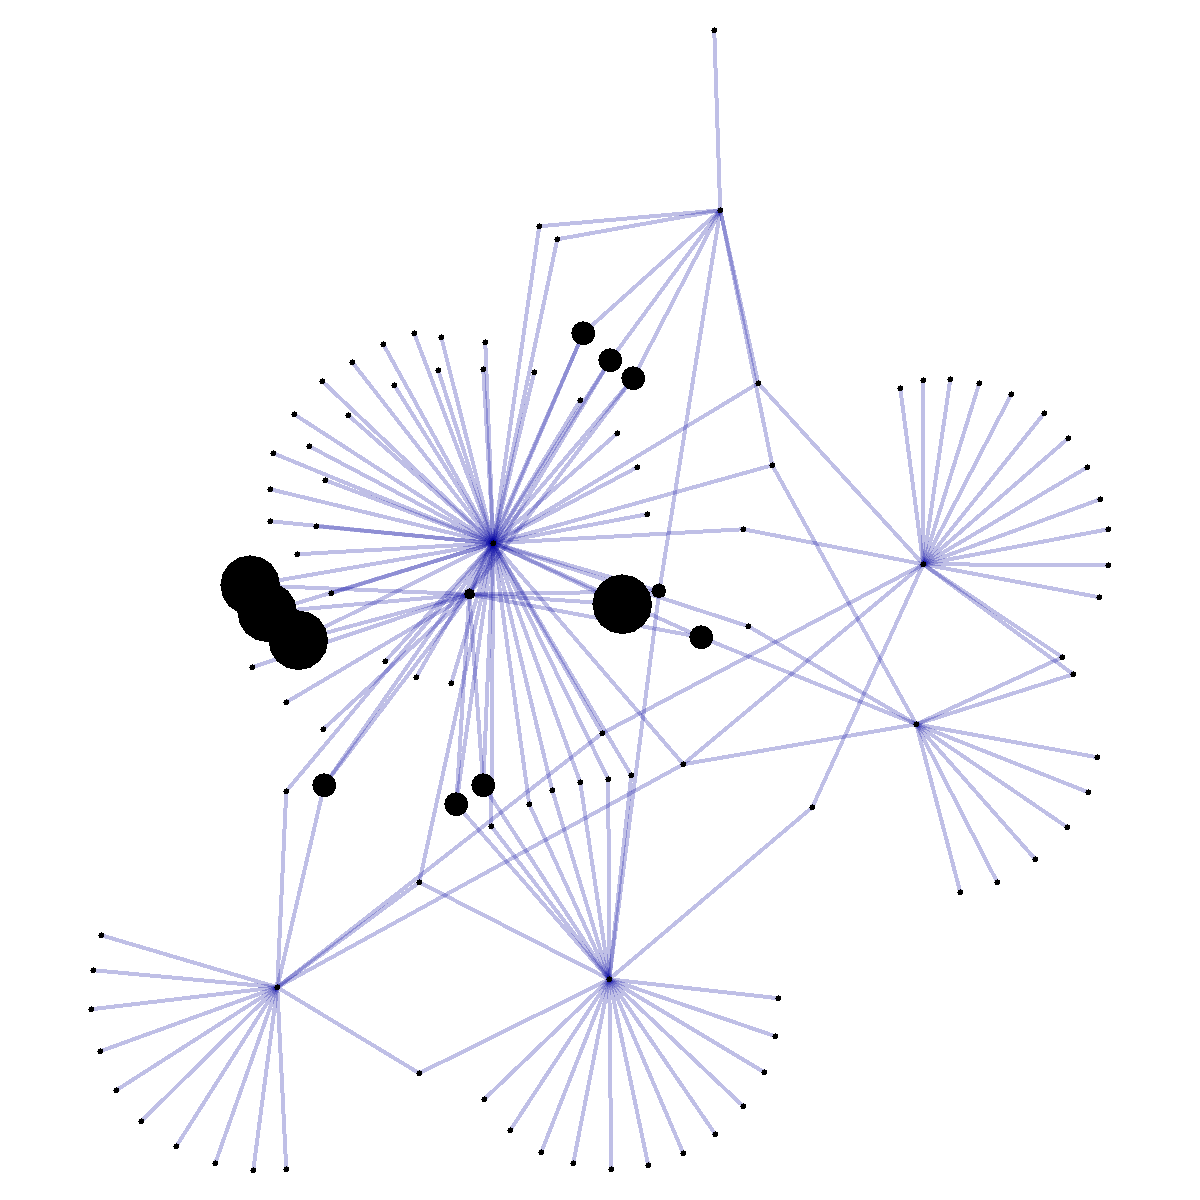
\includegraphics[height=5cm]{simplegraph_by_some_metrics3.png}
\caption{A simple graph with each node's diameter proportional to its \textsl{degree} (1), \textsl{betweenness centrality} (2), and \textsl{local clustering} (3).
In this particular graph, (1) and (2) show similar characteristics (greater value for more ``central'' nodes), whereas local clustering is significantly different.}
\label{fig:simplegraph_by_some_metrics}
\end{figure}


A common alternative for disconnected graphs is to compute \textsl{Harmonic centrality}.
It has similar meaning to closeness centrality, and a similar definition.

\begin{definition}[Harmonic centrality]\label{def:harmonic_centrality}
    \[HC(v) \eqdef \sum_{i \neq v} \frac{1}{d(v, i)}\]
    with $1 / d(v, i) = 0$ for disconnected nodes $v, i$ (as in~\cite{MarchioriHarmonySmallworld2000}).
\end{definition}

Both \textsl{closeness} and \textsl{harmonic centrality} require the computation of distances between all pairs of nodes.
I used an implementation of the Floyd–Warshall algorithm~\cite{FloydAlgorithm97Shortest1962} of time complexity $O({\left\lvert V \right\rvert}^3)$.
An alternative would be running Dijkstra's algorithm~\cite{dijkstra1959note} with time complexity $O({\left\lvert V \right\rvert}^2)$ starting in each node.

\todo{consider Seidel's APD algorithm, od Dijkstra}

\subsubsection{Ego network measures}

Ego networks are local subgraphs centered around a particular node in the network.
Step-$n$ ego network (also called ego-$n$ network) of a node $v$ is a subgraph including $v$ (the \textsl{ego} node), all nodes reachable from $v$ in at most $n$ hops (the \textsl{alter} nodes), and all edges among these (see \autoref{fig:ego_network}).
For simplicity, $\ego_n$ below are defined just as a subset of nodes $V$.

\begin{definition}[ego-$\mathbf{n}$ network]
    For a graph $G = (V, E)$, define inductively $\ego_n : V \rightarrow \mathcal{P}(V)$:
    \begin{align*}
        \ego_0(v) &\eqdef \left\{\, v \, \right\} \\
        \forall n \in \mathbb{N}.\ \ego_{n+1} (v) &\eqdef \ego_n \cup \Set{v' \in V}{ \exists v'' \in \ego_n(v).\ (v', v'') \in E }
    \end{align*}
\end{definition}

\begin{figure}
    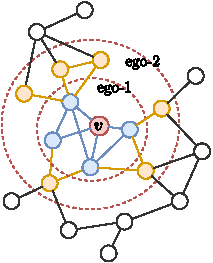
\includegraphics[height=5.5cm]{ego_network.pdf}
    \caption{An illustration of ego-$1$ and ego-$2$ networks of a node $v$}
    \label{fig:ego_network}
\end{figure}


Ego metrics are node metrics whose value depend only on properties of local ego network(s).
I chose and implemented 3 interesting ego metrics used also in The Paper.

\begin{definition}[ego-$\mathbf{1}$ edges]
    \[ E\mathit{1}E (v) = \left\lvert \Set{(v', v'') \in E}{ v' \in \ego_1(v) \wedge v'' \in \ego_1(v) } \right\rvert \]
\end{definition}

\begin{definition}[ego-$\mathbf{2}$ nodes]
    \[ E\mathit{2}N (v) = \left\lvert \ego_2(v) \right\rvert \]
\end{definition}

\begin{definition}[ego-$\mathbf{1/2}$ nodes ratio]
    \[ ER(v) = \frac{ \left\lvert \ego_1(v) \right\rvert }{ \left\lvert \ego_2(v) \right\rvert } \]
\end{definition}

\textsl{Local clustering} is also a common node metric, measuring the proportion of existing and all possible edges among neighbours of $v$, defined as in~\cite{WattsCollectiveDynamicsSmallworld1998}.
Following that, \textsl{redundancy} node metric is defined as the extent that $v$'s neighbours are adjacent to each other as well, according to~\cite{borgatti1997structural}.
\begin{definition}[Local clustering]
    Let $k = \deg(v)$, the degree of $v$, then
    \[
        LC(v) \eqdef
        \begin{dcases}
            0, &\text{if } k = 0,1 \\
            \frac{ \left\lvert \Set{ (v', v'') \in E }{ v' \in \ego_1(v) \wedge v'' \in \ego_1(v) } \right\rvert }{ k (k-1) / 2 } \quad &otherwise
        \end{dcases}
    \]

\end{definition}

\begin{definition}[Redundancy]
    \[ R(v) \eqdef LC (v) \times (\deg(v) - 1) \]

    Note that for $k \leq 1$, $LC(v) = R(v) = 0$.
\end{definition}

\subsubsection{Page rank}

A different, interesting node metric is \textsl{PageRank}~\cite{BrinAnatomyLargescaleHypertextual1998}, first developed for Google Search to rate the importance of websites.
For brevity, the full definition is not included here.
I used an implementation of PageRank that is described in~\cite{ilprints422}.


%\subsubsection{Eigenvector centrality}
%
%\subsubsection{Katz centrality}
%- not used much recently
%
%\subsubsection{PageRank}
%= Katz centrality, but divide each vertex's contribution by its out-degree
%
%\subsubsection{Hyperlink-induced topic search (HITS)}
%Hubs and authorities, by Kleinberg

% from GraphStream
%
%\subsubsection{CommunityMeasure}
%- Modularity\\
%- Community Distribution\\
%- CommunityRelativeMeasure $\rightarrow$ NormalizedMutualInformation $\rightarrow$ VariationOfInformation
%
%\subsubsection{Eccentricity}
%
%\subsubsection{Surprise measure}
%

\subsection{Ranking}

\todo{maybe move to~\nameref{sec:methods}}

%\begin{definition}[Preorder]
%    Binary relation $\sqsubseteq$ on some set $P$ is a \textbf{preorder} iff it is reflexive and transitive, i.e.:
%    \begin{itemize}
%        \item $\forall a, b \in P.\ a \sqsubseteq a$ \tabto{7.3cm}(reflexivity)
%        \item $\forall a, b, c \in P.\ (a \sqsubseteq b \wedge b \sqsubseteq c) \implies a \sqsubseteq c$ \tabto{7.3cm}(transitivity)
%    \end{itemize}
%\end{definition}
%
%\begin{definition}[Total preorder]
%    A binary relation $\sqsubseteq$ on some set $P$ is a \textbf{total preorder} iff it is a preorder and a connex relation, i.e.:
%    \begin{itemize}
%        \item $\forall a, b, c \in P.\ (a \sqsubseteq b \wedge b \sqsubseteq c) \implies a \sqsubseteq c$ \tabto{7.3cm}(transitivity)
%        \item $\forall a, b \in P.\ a \sqsubseteq b \vee b \sqsubseteq a$ \tabto{7.3cm}(connexity, implies reflexivity)
%    \end{itemize}
%\end{definition}

\begin{definition}[Partial order]
    A binary relation $\sqsubseteq$ on some set $P$ is a \textbf{partial order} iff it is antisymmetric preorder, i.e.:
    \begin{itemize}
        \item $\forall a, b \in P.\ a \sqsubseteq a$ \tabto{7.3cm}(reflexivity)
        \item $\forall a, b, c \in P.\ (a \sqsubseteq b \wedge b \sqsubseteq c) \implies a \sqsubseteq c$ \tabto{7.3cm}(transitivity)
        \item $\forall a, b \in P.\ (a \sqsubseteq b \wedge b \sqsubseteq a) \implies a = b$ \tabto{7.3cm}(antisymmetry)
    \end{itemize}
\end{definition}

\begin{definition}[Total order]
    A binary relation $\sqsubseteq$ on some set $P$ is a \textbf{total order} iff it is a partial order and a connex relation, i.e.:
    \begin{itemize}
        \item $\forall a, b, c \in P.\ (a \sqsubseteq b \wedge b \sqsubseteq c) \implies a \sqsubseteq c$ \tabto{7.3cm}(transitivity)
        \item $\forall a, b \in P.\ (a \sqsubseteq b \wedge b \sqsubseteq a) \implies a = b$ \tabto{7.3cm}(antisymmetry)
        \item $\forall a, b \in P.\ a \sqsubseteq b \vee b \sqsubseteq a$ \tabto{7.3cm}(connexity, implies reflexivity)
    \end{itemize}
\end{definition}

A less-than-or-equal relation ($\leq$) on real numbers $\mathbb{R}$ is an example of a total order.

\begin{definition}[Ranking relation]
    A binary relation $\preceq$ on the set of nodes $V$ of some graph $G = (V, E)$ is a \textbf{ranking relation induced by a metric $M$ on a graph $G$} iff it is a total order satisfying:

    \[ \forall v_1, v_2 \in V.\ M(v_1) < M(v_2) \implies v_1 \preceq v_2 \]
\end{definition}

By convention, we can consider a ranking to be a bijection between nodes $V$ and the set $\integersto{\left\lvert V \right\rvert}$, with the associated integers being called \textbf{ranks}.
This definition basically means that ranking with respect to a metric is \textsl{a} ordering of nodes such that nodes with high metric values correspond to high ranks.

\begin{definition}[Ranking (vector)]
    A \textbf{ranking vector} $A^{\preceq}$, or a \textbf{ranking}, induced by a metric $M$ on a graph $G$ is a bijection $V \leftrightarrow \integersto{\left\lvert V \right\rvert}$ such that
    \[ \forall v_1, v_2 \in V.\ v_1 \preceq v_2 \implies A^{\preceq}(v_1) \leq A^{\preceq}(v_2), \]
    where $\preceq$ is a ranking relation of graph $G = (V, E)$ with respect to metric $M$.

    Also, allow $A^{M(G)}$ as a shortened notation of a ranking induced by the metric $M$ on the graph $G$.
    Therefore,
    \[ A^{M(G)} : V \leftrightarrow \integersto{\left\lvert V \right\rvert} \]
\end{definition}

Note, there may be multiple valid rankings if multiple nodes have the same metric value, in which case any mutual order of such nodes is permitted in the ranking.
A ranking just assigns each node a rank (or a position) such that it doesn't violate the ordering by metric values.
Also, note that each node must be assigned a \textsl{unique} rank, due to the antisymmetry property.

\todo{explain how ties are resolved (in The Paper: randomly)}

\todo{add graph figure with ranked nodes (either labels or node size by rank)}


\subsubsection*{Why do we need rankings of nodes?}

When studying robustness of graph metrics, we ultimately aim to assess how stable an analysis using metrics is, on a network coming from an ``imprecise'' source.
By an imprecise source I mean a way of obtaining datasets that may lead to different network each time it is obtained.
Essentially, networks from the real-world may depend on the measurement environment or on hyper parameters.

It is clear that values of most metrics will naturally change with changing graph structure.
So to measure robustness of a metric on a higher level, The Paper uses robustness measures which only depend on \textbf{ranking} of nodes with respect to values of the given metric.
This may then result in high stability of a metric which identifies similar sets of \textsl{most important} nodes (whatever that means for this metric) across more perturbed graphs, even if the exact values across those graphs are different.

\parspace

For example, in protein networks that we evaluate metrics on, the graph itself depends on the \textsl{confidence threshold}.
In particular, higher confidence thresholds generally lead to more sparse graphs.
Then, the degree of nodes will principally decrease with increasing confidence threshold, however, degree happens to be a relatively stable metric in general, which means the sets of highest-degree nodes will be relatively similar across graphs of similar thresholds.

For different datasets there may other hyper- or hidden parameters in the procedure of obtaining the graph.
The difference between graphs obtained from the same imprecise source are always some small perturbations that stable metrics should ideally be resilient to.

\subsection{Robustness}

At the highest level where metrics are functions (\autoref{eq:metric_type_def}), robustness measures can be regarded as functions from $\mathbb{M}$ (the domain of all metrics) to real numbers.
\begin{equation}
    \mathcal{R} \eqdef \mathbb{M} \Rightarrow \mathbb{R}
\end{equation}

There are two important points to be made.

\subsubsection*{Robustness is empirical}

First, the point of this dissertation is not to analyse the metrics purely as functions and thus reason about their robustness (which would indeed be difficult and not generalisable), instead, I analyse robustness \textbf{empirically}, by evaluating metrics on many graphs and deducing clues about how stable the values are across these multiple graphs.
More on this is in the~\nameref{sec:methods} section.

\subsubsection*{Per-graph robustness}

Secondly, as the robustness measures are calculated by evaluating metrics on graphs, the robustness values will inherently depend on the graphs chosen.
To mitigate this, one could theoretically analyse a metric on a huge set of all kinds of graphs (such as social networks, road networks, internet networks, protein interaction networks, etc.), but the two drawbacks are:
\begin{itemize}
    \item We can perhaps never construct a set covering all \textsl{kinds} of graphs, and that is in no way the point of this dissertation
    \item The robustness of metrics would be highly dependent on the particular set of graphs it is tested on, as one metric may be, in general, more stable on dense graphs, where another metric may be unstable.
\end{itemize}

For this reason, I will mainly consider and analyse \textbf{robustness} of a metric \textbf{on a certain graph}.
Hence, I will rather use this concept:
\begin{equation}
    \mathcal{R} \eqdef \mathbb{M} \times \mathbb{G} \Rightarrow \mathbb{R}
\end{equation}

Per-graph robustness is, indeed, not helpful in answering the question ``Which metrics can I rely on when analysing my custom dataset X?'' which is one of the main problems this project attempts to solve.
\begin{itemize}
    \item The Paper only calculates robustness by experiments on protein interaction networks (which presumably follow a similar structure), and then even dares to calculate the averaged robustness measures across a number of PINs.
    \item In my dissertation, instead of coming up with more-general results, I rather focused on designing a way to analyse robustness of metrics, and built a \textsl{tool} that can perform this analysis generally on any given graph.
\end{itemize}


\section{Methods}\label{sec:methods}

Taking the concepts defined in the~\nameref{sec:math_background} section, here I introduce methods that I used to build the \graffs tool.
In particular, this section will discuss mainly the following, in the theoretical framework:
\begin{itemize}
    \item discuss \textsl{datasets}, their kinds, and where to find them
    \item \textsl{small perturbations} on graphs, and ways to generate \textsl{perturbed} graphs
    \item applying metrics to perturbed graphs
    \item define overall rank, $k$-similarity, $\alpha$-relaxed $k$-similarity
    \item ways to quantify \textsl{robustness} of metrics
\end{itemize}

\subsection{Datasets}\label{sec:datasets}

Later in this section I present different kinds of publicly available graph datasets used in this project.
In my work I distinguish two types of networks: scored and unscored.

\todo{add citations for individual datasets used}

\subsubsection{Scored networks}\label{sec:scored_networks}

In scored networks, the edges are weighted, with each weight, also called the \textbf{score}, representing the likelihood that the edge is true in the real world.

The score is usually a real value between $0$ and $1$.

\begin{wrapfigure}[11]{R}{0.24\textwidth}
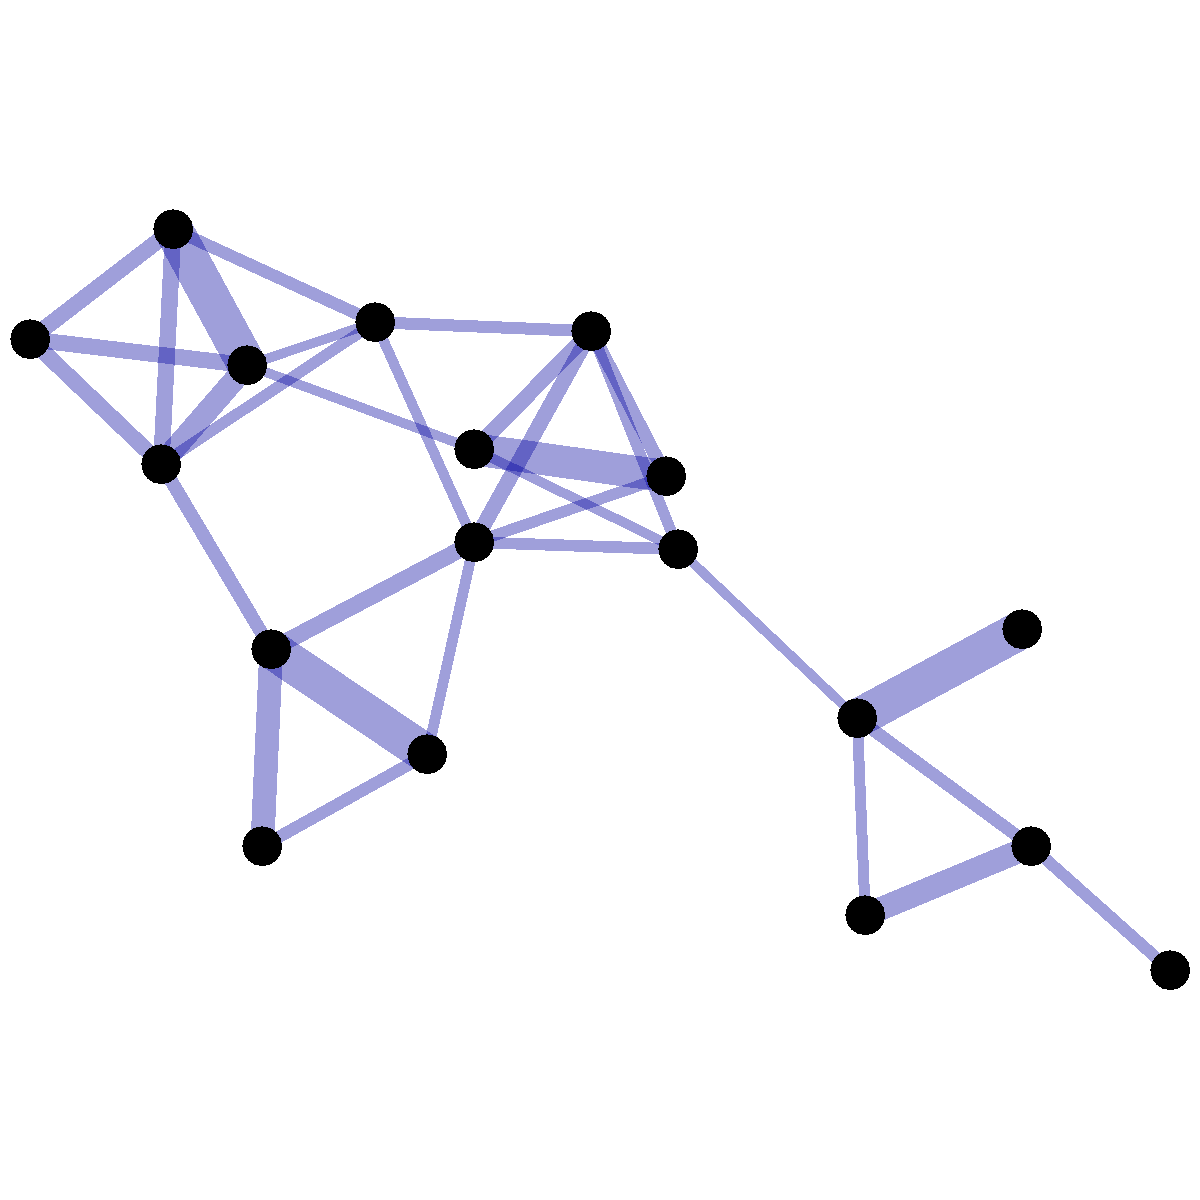
\includegraphics[width=\linewidth,trim=0 3.4cm 0 3.2cm,clip,angle=90,origin=c]{graph_example_scored_edges.png}
\caption{A tiny subgraph of the \texttt{ecoli} dataset with the width of edges proportional to their scores}
\label{fig:graph_example_scored_edges}
\end{wrapfigure}


Scored protein networks are a good example of scored networks.
\autoref{fig:graph_example_scored_edges} shows a small subgraph of the \textsl{Escherichia coli} dataset from the~\nameref{sec:string_database} where edges in the figures are drawn with the width proportional to their weight.

Scored networks are useful for metric robustness analysis because they naturally provide a way to introduce perturbations to the networks -- by adjusting the confidence threshold.

Using a scored network as-is just by discarding the confidence score is often unacceptable as a large proportion of the network's edges with close-to-zero confidence are likely to be false positives.
Obtaining a functional network from an almost fully connected clique needs starting with a reasonable confidence threshold.
Scored databases often state what is the reasonable range of the confidence scores.

\subsubsection{Unscored networks}

Unscored networks are just unweighted graphs, therefore not conveying the information about confidence of edges.

When we apply a confidence threshold to a scored network, discarding the scores, the resulting subgraph with a filtered set of edges is an unscored network.

\parspace

Although the \graffs tool built is universal and is not bound to any kind of dataset, I chose a number of datasets to work with to demonstrate the concept.

There are multiple online sources providing interesting network datasets.

\subsubsection{STRING database}\label{sec:string_database}

\textit{STRING}\cite{Szklarczyk2019} is an open database of scored interactions between proteins.
At the time of writing, the database contains over 24M different proteins from over 5K organisms, accounting for over $2 * 10^9$ interactions.

Considering the whole graph as an input for this project would be unsuitable because of its size, but for the evaluation, sub-graphs of proteins of only certain organisms will be used.

Note that, generally, one cannot just consider a subgraph of a source graph (such as sub-graph of a social network), because the generated sub-graph doesn't have a meaning, and its characteristic heavily depend on how the graph was generated (for example, in a social network with communities, taking $n$ random nodes adjacent to a certain node would likely result in a more dense graph than taking $n$ random nodes of the whole graph).
However, we can generate subgraphs of the whole STRING database by considering only proteins of concrete organism.
Such full-organism networks then describe interactions of proteins within that organism.

In my work, I evaluate robustness on the following datasets taken from the STRING database:
\begin{itemize}
    \item Plasmodium vivax (\textsl{pvivax}) -- 3255 nodes, 344691 edges
    \item Escherichia coli (\textsl{ecoli}) -- 4144 nodes, 583440 edges
    \item Saccharomyces cerevisiae (\textsl{yeast}) -- 6418 nodes, 939998 edges
\end{itemize}

The datasets are too large to be visualised as graphs.
\todo{Figure X} presents the degree distribution of the datasets.
\todo{Figure Y} shows the effect of thresholding on the average degree.

The STRING database also provides guidance on what the reasonable ranges of the score values are, with the score being `the approximate probability that a predicted link exists between two enzymes (proteins)':
\begin{itemize}
    \item low confidence -- 0.15 (or better)
    \item medium confidence -- 0.4
    \item high confidence -- 0.7
    \item highest confidence -- 0.9
\end{itemize}

\subsubsection{Stanford Large Network Dataset Collection}

The \textit{Stanford Large Network Dataset Collection}\cite{Large2016} provides open datasets obtained from real-world data such as social networks, citation networks, web graphs, internet networks, road networks and many more.

\todo{list used datasets}

\subsubsection{KONECT datasets}

Another dataset collection: The Koblenz Network Collection (KONECT)~\cite{Kunegis2013} provides access to hundreds of network datasets of various types.
Its covers diverse areas such as `social networks, hyperlink networks, authorship networks, physical networks, interaction networks, and communication networks'.

\todo{list used datasets}

\subsection{Perturbing graphs}\label{sec:perturbing_graphs}

The goal of the dissertation is to empirically study how resilient a graph metric is to small perturbations in an input graph.
This only relates to graphs that ``approximate'' the observed real-world structures, and are not their exact representation.
For example, thresholded protein networks are not exact due to measurements.
An online social network may not represent all relationships between people exactly because not all people or relationships may be registered, or some may be obsolete.
Analysing robustness of a metric then means studying how much different the metric values \textsl{could be} if we performed the same experiment on other datasets coming from the same source -- datasets possibly measured by different techniques, at different times, with different methodology, or in a different universe.

However, when studying a graph, usually, we are only given one dataset to work with, i.e. exactly one ``inexact'' structure of the real world.
To simulate having multiple similar graphs, we need ways to ``generate'' those new similar graphs from a given input graph.
I will refer to them as \textbf{perturbed} graphs generated from a \textbf{base} graph.
Here, ``similar'' means that they convey the same real-world structure.

At the high level, a graph generator $\xi$ is a function that takes a graph $G$ and a number $n$ and generates a sequence of $n$ graphs based on $G$.
\begin{equation}
    \mathlarger{\xi}(G) \generates{n} G_1, G_2, \dots, G_n
\end{equation}

Note: the~\nameref{sub:rank_continuity} robustness measure compares pairs of consecutively generated graphs (e.g. graphs thresholded at consecutive confidence threshold), that is why we define graph generator to output a sequence of graphs instead of a set.

The exact value of $n$ is conceptually unimportant and is discussed in the~\nameref{ch:evaluation} chapter.

\parspace

For measuring metric robustness it will be beneficial to know matching between multiple graphs coming from the same dataset, or in other words to preserve identity of nodes across such graphs.
So, define:

\begin{definition}[Graph matching]
    \label{def:graph_matching}
    Given two generated graphs graphs $G_1 = (V_1, E_1)$ and $G_2 = (V_2, E_2)$ derived from the same network, define \textbf{graph matching}, $\leftrightsquigarrow$, to be a bijection between $V_1, V_2$ such that
    \begin{equation}
        \forall v_1 \in V_1, \forall v_2 \in V_2.\quad v_1 \leftrightsquigarrow v_2\quad\text{iff}\quad \begin{array}{l}
                                                                                                            v_1, v_2\ \text{correspond to the same }\\\text{node in the base graph}
        \end{array}
    \end{equation}
\end{definition}

\subsubsection{Thresholding scored networks}

Various methods were proposed to choose a good baseline threshold, from fixing the value upfront\cite{MeunierAgerelatedChangesModular2009} or after examining a range of values\cite{vanWijkComparingBrainNetworks2010,HorstmannStateDependentProperties2010}, through maximising the threshold given some constraints\cite{BassettAdaptiveReconfigurationFractal2006}, to choosing a value optimising some criterion such as classification rate\cite{ZaninOptimizingFunctionalNetwork2012}.
However, the confidence threshold value is still a hyper-parameter of the graph-obtaining process and robust metrics should respond similarly to all reasonable values of the chosen threshold.

For scored networks, such as protein networks, we can generate perturbed graphs by considering different confidence thresholds (in a reasonable range) of the same scored network.
Resulting is a sequence of graphs with decreasing density as the threshold increases.

Define a \textbf{linear thresholding} graph generator, given a minimum threshold $t_0$ and a maximum threshold $t_1$, as follows:
\begin{align}
    &\mathlarger{^T \mathlarger{\xi}}_{t_0}^{t_1}(G) \generates{n} (V, E')~\text{for}~i\in \integersto{n}, \\[10pt]
    \text{where}~&E' = \Set{(v_1, v_2)\in E}{ c(v_1, v_2) > t_0 + \frac{i}{n - 1}(t_1 - t_0) }, \nonumber \\
    &G = (V, E)~\text{is the base graph}, \nonumber \\
    &c(v_1, v_2)~\text{is the confidence score of the edge $v_1\,\text{---}\,v_2$} \nonumber
\end{align}

\todo{generate an array of ~8 linearly thresholded graphs to demonstrate this effect}

\subsubsection{Randomly deleting edges}\label{sec:randomly_removing_edges}

For unscored networks, we need to devise another way to simulate the effect of obtaining multiple similar graphs of the same real-world structure.

One study in a similar context~\cite{BorgattiRobustnessCentralityMeasures2006} proposes four kinds of random error:
\begin{itemize}[topsep=5pt]
    \item deleting edges,
    \item deleting nodes,
    \item adding edges,
    \item adding nodes (and connecting them to the graph by random edges),
\end{itemize}
all with a given small percentage of nodes or edges to be affected.

The two adding methods (adding edges and adding nodes) both depend on the particular distribution for sampling new edges.
We cannot easily generalise this pattern as different graphs have various structures and so no general edge sampling distribution would likely suit all graphs.
Hence, I will stick to random deletion.

Further, deleting nodes would possibly introduce more drastic and uncontrollable perturbations in densely connected networks, because deleting a high-degree node means deleting many edges -- a more extreme change in the structure than deleting a low-degree node.
One could mitigate this by sampling nodes to delete according some clever non-uniform distribution, but then the distribution itself would be another hyper-parameter that can itself condition robustness measures.

Another argument against using node deletion is that the 3 robustness measures proposed by The Paper are based on identifying and comparing sets of the most important nodes with respect to a given metric.
Thus, random node deletion could have a significant bias in these robustness measures, whereas edge deletion does not pose direct bias the measures (only indirectly, by affecting metric values).

For the reasons above, I decided to stick with random edge deletion.

\parspace

Define an \textbf{edge removing} graph generator, given a proportion of edges to delete $\alpha$ (deletion rate), as follows:
\begin{align}
    &\mathlarger{^{ER} \mathlarger{\xi}}_\alpha(G) \ \overset{n}{\hookrightarrow}\ (V, E')~\text{for}~i\in \integersto{n}, \label{eq:edge_removing_generator}\\[10pt]
    \text{where}~&E' = \Set{ e \in E }{ \chi_e > \alpha }, \nonumber \\
    &\forall e \in E.\ \chi_e\sim\mathcal{U}(0,1) \nonumber
\end{align}

\todo{generate an array of ~8 linearly thresholded graphs to demonstrate this effect}

Unlike linear thresholding, edge removing is applicable to unscored networks (and to scored networks after applying a threshold).
However, in practice it is useful to specify an \textsl{initial threshold} so that this generator can work on scored networks too, by turning them into unscored.
Note that keeping all edges and purely discarding the confidence scores would be detrimental, as low-scored edges would make scored networks falsely dense.

\subsection{Evaluating metrics}\label{sec:evaluating_metrics}

To study how values of a metric change as we do small perturbations to the input graph, we first evaluate the metric on a number of perturbed graphs and then study the values across all graphs.

Given a metric $M$, a base graph $G_0$, a graph generator $\xi$, and the number of perturbed graphs $n$, let \textbf{metric evaluation} refer to the application of a metric to a sequence of generated graphs:
\begin{align}
    M \overset{\mathlarger{\xi}}{\vdash} G_0 &\generates{n} M(G_1), M(G_2), \dots, M(G_n), \\[10pt]
    \text{with}\qquad \mathlarger{\xi}(G_0) &\generates{n} G_1, G_2, \dots, G_n \nonumber
\end{align}

Finally, define \textsl{overall ranking} on a sequence of perturbed graphs that is calculated by first averaging node ranks over all induced rankings, and then ranking the averaged values.

\begin{definition}[Overall ranking]
    \label{def:overall_ranking}
    An \textbf{overall ranking} $A^*$ of a metric $M$ on $n$ perturbed graphs generated using $\xi$ from a base graph $G_0$, is defined as:

    \begin{align*}
        &\mathlarger{A^*}\!\left( M \mid G_0, \xi, n \right) = A^{\operatorname{Avg}(G_0)} ,\\[5pt]
        \text{where}~&\operatorname{Avg}(G) :\ \forall v \in V.\ v \,\mapsto\, \frac{1}{n} \sum_{i=1}^n A^{M(G_i)}(v)\, , \\
        &\begin{aligned}
             \text{where}~\,&\xi(G) \generates{n} G_1, \dots, G_n\,, \\
             & G = (V, E)
        \end{aligned}
    \end{align*}
\end{definition}

In the definition, $A^{M(G_i)}$ is the ranking induced on one generated graph.
For each node $v$, we calculate the average of $v$'s rank across all rankings, and call it a metric $\operatorname{Avg}$ (because it maps each node to a value).
Then the overall ranking is just the ranking of the locally defined $\operatorname{Avg}$ metric.

\subsection{Robustness measures}\label{sec:robustness_measures}

In this section I define the 3 robustness measures proposed by The Paper: rank continuity, rank identifiability, and rank instability.
Then I explain how I extended two of the measures from scored networks to unscored networks.\todo{extend these to unscored networks}

The Paper argues that in the context of bioinformatics, metrics are often used to identify key nodes of graphs, therefore it is natural to focus on the highest ranking nodes only.
This is also true for networks that are just too large for each node to be inspected individually\citeneeded.
Hence, in principle, the three robustness measures test how reliably a metric can identify a certain number of highest-ranked nodes across multiple perturbed graphs.


For that, I will first define the notion of $k$-similarity and $\alpha$-relaxed $k$-similarity, as proposed in The Paper.
Both similarities quantify a relationship between two rankings with meaning similar to rank correlation coefficient, but take into account the highest-ranked nodes only.

\begin{definition}[$\bm{k}$-similarity]
    \label{def:k_similarity}
    The \textbf{$\bm{k}$-similarity} of two rankings $A_\theta, A_\mu$ is the overlap between their $100k\%$ highest ranking nodes:
    \[ M_k(A_\theta, A_\mu \mid k) = \frac{\left\lvert \Set{v \in V^{\cap}}{ A_\theta(v) > N(1-k) \wedge A_\mu(v) > N(1-k) } \right\rvert}{Nk} \]
    where $k \in \left( 0, 1 \right]$ and $V^{\cap}$ is the intersection of domains of $A_\theta, A_\mu$.
\end{definition}

Note that this measure of rank similarity is symmetric.
Also, as none of the used graph generator methods alter the set of nodes, we have $V_\theta = V_\mu = V^{\cap}$ (the sets of nodes of the two graphs will always be equal).

The following $\alpha$-relaxed $k$-similarity accounts for situations where the two rankings don't carry the same meaning and are interpreted differently.

\begin{definition}[$\bm{\alpha}$-relaxed $\bm{k}$-similarity]
    \label{def:alpha_relaxed_k_similarity}
    The \textbf{$\bm{\alpha}$-relaxed $\bm{k}$-similarity} of two rankings $A_\theta, A$ is the proportion of the $100k\%$ highest ranking nodes in $A$ which are also within $100k\bm{a}\%$ highest ranking nodes in $A_\theta$:
    \[ M_k^\alpha(A_\theta, A \mid k) = \frac{\left\lvert \Set{v \in V^{\cap}}{ A_\theta(v) > N(1-k\bm{\alpha}) \wedge A_\mu(v) > N(1-k) } \right\rvert}{Nk} \]
    where $\alpha > 0$, $k, k\alpha \in \left( 0, 1 \right]$ and $V^{\cap}$ is the intersection of domains of $A_\theta, A$.
\end{definition}

For example, if $A_\theta$ is obtained by ranking a perturbed graph and $A$ is an overall ranking (of multiple perturbed graphs), relaxed $k$-similarity may be used to identify whether the top 10 nodes overall, i.e. in $G$, are among the top 20 for the particular observed threshold, i.e. in $G_\theta$.

\todo{other robustness measures:~\cite{BorgattiRobustnessCentralityMeasures2006}}

\todo{The Paper also refers to:} Rank similarity typically measured by a rank correlation coefficient such as Spearman or Kendall.

\parspace

The following three rank robustness measures are defined given a metric $M$, a base graph $G_0$, a graph generator $\xi$, and the number of perturbed graphs $n$

\subsubsection{Rank continuity}\label{sub:rank_continuity}

Speaking of scored networks, rank continuity of a metric is the similarity between rankings induced at consecutive thresholds.

\begin{definition}[Rank continuity]\label{def:rank_continuity}
    \ldots
\end{definition}

\ldots

\subsubsection{Rank identifiability}

\subsubsection{Rank instability}

\begin{definition}[Rank instability]
    \newcommand*{\args}{\left(M \mid G, \xi, n \right)}\newcommand*{\astar}{A^*\!\args}
    The \textbf{rank instability} measure is defined as:

    \begin{flalign}
        &\operatorname{rank\ instability} \args \eqdef \frac{1}{\left\lvert U \right\rvert}\, \mathlarger{\sum}_{v \in U} \frac{range(v)}{n} & \\[10pt]
        \text{where }\ & A = \astar \quad \text{(an overall ranking, by Definition~\ref{def:overall_ranking})}, \nonumber \\
        & U = \Set{v \in V}{A(v) > 99\%n}, \nonumber \\[2pt]
        & range : \begin{array}[t]{l}
                      V \to \mathbb{R}\\ v \,\mapsto\,  \max\limits_{i \in \integersto{n}} \left( A^{M(G_i)}(v) \right)  -  \min\limits_{i \in \integersto{n}} \left( A^{M(G_i)}(v) \right)\ ,
        \end{array} \nonumber \\
        & G = (V, E) \nonumber
    \end{flalign}
\end{definition}

In the definition, $U$ is the set of the $1\%$ highest ranked nodes according to the overall ranking $A^*\!\left(M \mid G, \xi, n \right)$.
Then, for each node $v$, we calculate a range of \textsl{ranks} that the node holds across the generated graphs $G_1$ to $G_n$.
Finally, the rank instability measure is calculated as the average scaled range for the $1\%$ highest ranked nodes in $U$.

\parspace

\todo{include some cool figures to demonstrate the three robustness measures}


